\documentclass{standalone}
\usepackage{tikz}
\usetikzlibrary{patterns, positioning}

\begin{document}
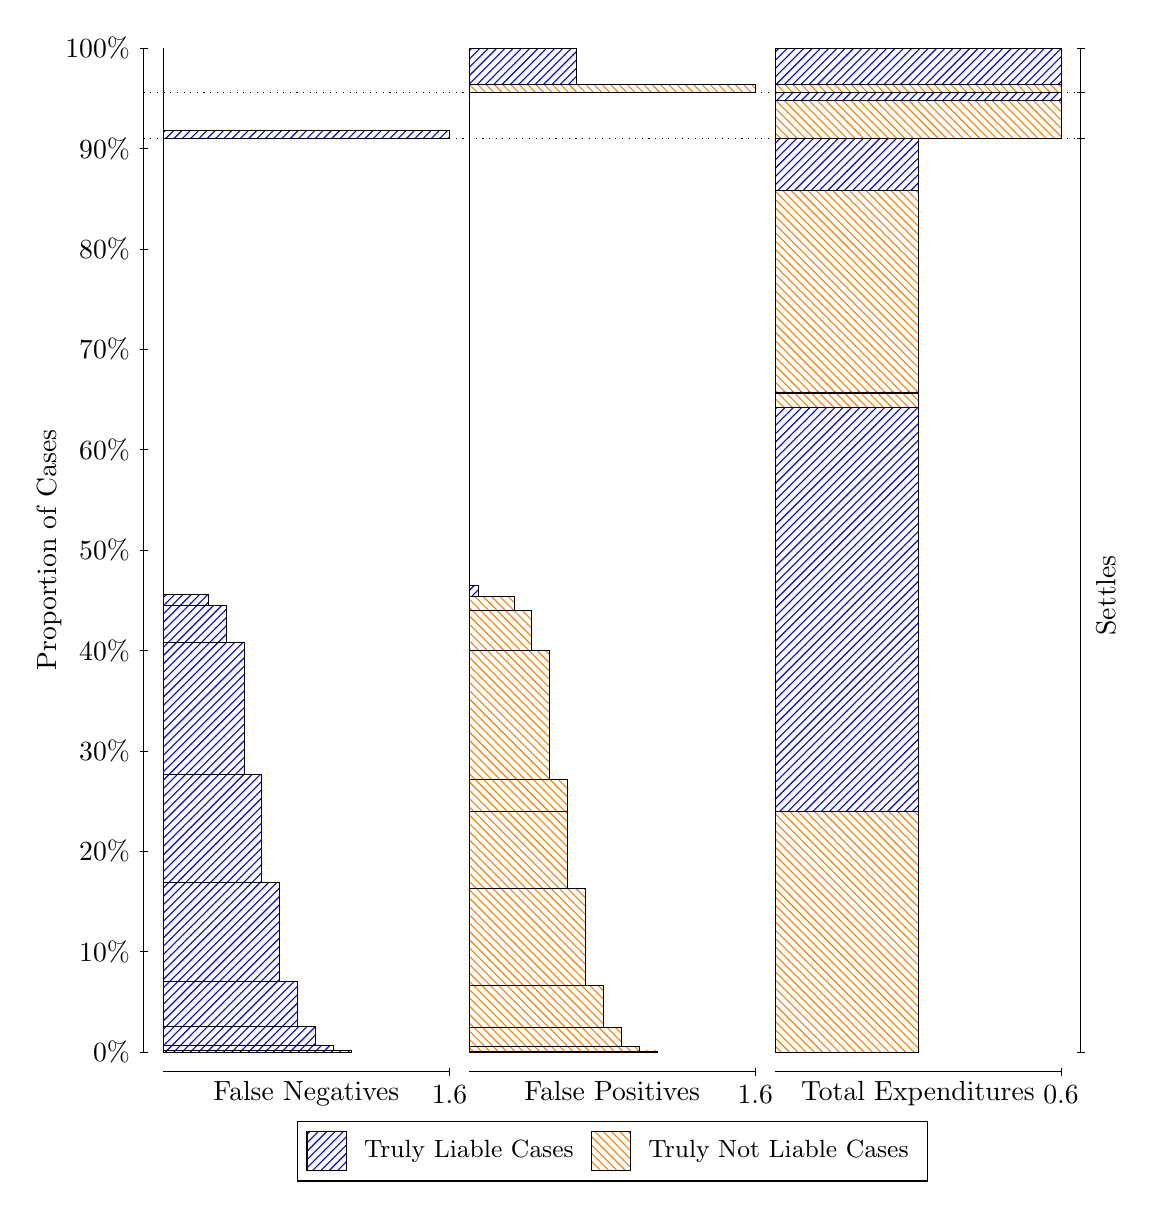
\begin{tikzpicture}
\draw[black, very thin] (1.5,1.75) -- (1.5,14.5);
\node[rotate=90, anchor=center] at (0.3, 8.125) {Proportion of Cases};
\draw[black, very thin] (1.45,1.75) -- (1.55,1.75);
\node[anchor=east] at (1.45, 1.75) {0\%};
\draw[black, very thin] (1.45,3.025) -- (1.55,3.025);
\node[anchor=east] at (1.45, 3.025) {10\%};
\draw[black, very thin] (1.45,4.3) -- (1.55,4.3);
\node[anchor=east] at (1.45, 4.3) {20\%};
\draw[black, very thin] (1.45,5.575) -- (1.55,5.575);
\node[anchor=east] at (1.45, 5.575) {30\%};
\draw[black, very thin] (1.45,6.85) -- (1.55,6.85);
\node[anchor=east] at (1.45, 6.85) {40\%};
\draw[black, very thin] (1.45,8.125) -- (1.55,8.125);
\node[anchor=east] at (1.45, 8.125) {50\%};
\draw[black, very thin] (1.45,9.4) -- (1.55,9.4);
\node[anchor=east] at (1.45, 9.4) {60\%};
\draw[black, very thin] (1.45,10.675) -- (1.55,10.675);
\node[anchor=east] at (1.45, 10.675) {70\%};
\draw[black, very thin] (1.45,11.95) -- (1.55,11.95);
\node[anchor=east] at (1.45, 11.95) {80\%};
\draw[black, very thin] (1.45,13.225) -- (1.55,13.225);
\node[anchor=east] at (1.45, 13.225) {90\%};
\draw[black, very thin] (1.45,14.5) -- (1.55,14.5);
\node[anchor=east] at (1.45, 14.5) {100\%};

\draw[black, very thin] (13.4,1.75) -- (13.4,14.5);
\draw[black, very thin] (13.35,1.75) -- (13.45,1.75);
\node[anchor=west] at (13.35, 1.75) {};
\draw[black, very thin] (13.35,13.349) -- (13.45,13.349);
\node[anchor=west] at (13.35, 13.349) {};
\draw[black, very thin] (13.35,13.937) -- (13.45,13.937);
\node[anchor=west] at (13.35, 13.937) {};
\draw[black, very thin] (13.35,14.5) -- (13.45,14.5);
\node[anchor=west] at (13.35, 14.5) {};

\draw[black, very thin, pattern color=blue, pattern=north east lines] (1.75,1.75) rectangle (4.1344,1.768);
\draw[black, very thin, pattern color=blue, pattern=north east lines] (1.75,1.768) rectangle (3.9073,1.8308);
\draw[black, very thin, pattern color=blue, pattern=north east lines] (1.75,1.8308) rectangle (3.6802,2.0769);
\draw[black, very thin, pattern color=blue, pattern=north east lines] (1.75,2.0769) rectangle (3.4531,2.6513);
\draw[black, very thin, pattern color=blue, pattern=north east lines] (1.75,2.6513) rectangle (3.226,3.9019);
\draw[black, very thin, pattern color=blue, pattern=north east lines] (1.75,3.9019) rectangle (2.999,5.2766);
\draw[black, very thin, pattern color=blue, pattern=north east lines] (1.75,5.2766) rectangle (2.7719,6.9557);
\draw[black, very thin, pattern color=blue, pattern=north east lines] (1.75,6.9557) rectangle (2.5448,7.4216);
\draw[black, very thin, pattern color=blue, pattern=north east lines] (1.75,7.4216) rectangle (2.3177,7.5617);
\draw[black, very thin, pattern color=orange, pattern=north west lines] (1.75,7.5617) rectangle (1.75,13.349);
\draw[black, very thin, pattern color=blue, pattern=north east lines] (1.75,13.349) rectangle (5.3833,13.455);
\draw[black, very thin, pattern color=orange, pattern=north west lines] (1.75,13.455) rectangle (1.75,13.937);
\draw[black, very thin, pattern color=orange, pattern=north west lines] (1.75,13.937) rectangle (1.75,14.043);
\draw[black, very thin, pattern color=blue, pattern=north east lines] (1.75,14.043) rectangle (1.75,14.5);
\draw[black, very thin, pattern color=orange, pattern=north west lines] (5.6333,1.75) rectangle (8.0177,1.7645);
\draw[black, very thin, pattern color=orange, pattern=north west lines] (5.6333,1.7645) rectangle (7.7906,1.8209);
\draw[black, very thin, pattern color=orange, pattern=north west lines] (5.6333,1.8209) rectangle (7.5635,2.064);
\draw[black, very thin, pattern color=orange, pattern=north west lines] (5.6333,2.064) rectangle (7.3365,2.5995);
\draw[black, very thin, pattern color=orange, pattern=north west lines] (5.6333,2.5995) rectangle (7.1094,3.8283);
\draw[black, very thin, pattern color=orange, pattern=north west lines] (5.6333,3.8283) rectangle (6.8823,4.8022);
\draw[black, very thin, pattern color=orange, pattern=north west lines] (5.6333,4.8022) rectangle (6.8823,5.2107);
\draw[black, very thin, pattern color=orange, pattern=north west lines] (5.6333,5.2107) rectangle (6.6552,6.8534);
\draw[black, very thin, pattern color=orange, pattern=north west lines] (5.6333,6.8534) rectangle (6.4281,7.363);
\draw[black, very thin, pattern color=orange, pattern=north west lines] (5.6333,7.363) rectangle (6.201,7.5373);
\draw[black, very thin, pattern color=blue, pattern=north east lines] (5.6333,7.5373) rectangle (5.7469,7.6775);
\draw[black, very thin, pattern color=blue, pattern=north east lines] (5.6333,7.6775) rectangle (5.6333,13.349);
\draw[black, very thin, pattern color=orange, pattern=north west lines] (5.6333,13.349) rectangle (5.6333,13.831);
\draw[black, very thin, pattern color=blue, pattern=north east lines] (5.6333,13.831) rectangle (5.6333,13.937);
\draw[black, very thin, pattern color=orange, pattern=north west lines] (5.6333,13.937) rectangle (9.2667,14.043);
\draw[black, very thin, pattern color=blue, pattern=north east lines] (5.6333,14.043) rectangle (6.9958,14.5);
\draw[black, very thin, pattern color=orange, pattern=north west lines] (9.5167,1.75) rectangle (11.333,4.8022);
\draw[black, very thin, pattern color=blue, pattern=north east lines] (9.5167,4.8022) rectangle (11.333,9.9394);
\draw[black, very thin, pattern color=orange, pattern=north west lines] (9.5167,9.9394) rectangle (11.333,10.114);
\draw[black, very thin, pattern color=blue, pattern=north east lines] (9.5167,10.114) rectangle (11.333,10.132);
\draw[black, very thin, pattern color=orange, pattern=north west lines] (9.5167,10.132) rectangle (11.333,12.693);
\draw[black, very thin, pattern color=blue, pattern=north east lines] (9.5167,12.693) rectangle (11.333,13.349);
\draw[black, very thin, pattern color=orange, pattern=north west lines] (9.5167,13.349) rectangle (13.15,13.831);
\draw[black, very thin, pattern color=blue, pattern=north east lines] (9.5167,13.831) rectangle (13.15,13.937);
\draw[black, very thin, pattern color=orange, pattern=north west lines] (9.5167,13.937) rectangle (13.15,14.043);
\draw[black, very thin, pattern color=blue, pattern=north east lines] (9.5167,14.043) rectangle (13.15,14.5);
\draw[black, dotted] (1.5,13.349) -- (13.4,13.349);
\draw[black, dotted] (1.5,13.937) -- (13.4,13.937);
\draw[black, very thin] (1.75,1.5) -- (5.3833,1.5);
\node[anchor=north] at (3.5667, 1.5) {False Negatives};
\draw[black, very thin] (5.3833,1.45) -- (5.3833,1.55);
\node[anchor=north] at (5.3833, 1.45) {1.6};

\draw[black, very thin] (5.6333,1.5) -- (9.2667,1.5);
\node[anchor=north] at (7.45, 1.5) {False Positives};
\draw[black, very thin] (9.2667,1.45) -- (9.2667,1.55);
\node[anchor=north] at (9.2667, 1.45) {1.6};

\draw[black, very thin] (9.5167,1.5) -- (13.15,1.5);
\node[anchor=north] at (11.333, 1.5) {Total Expenditures};
\draw[black, very thin] (13.15,1.45) -- (13.15,1.55);
\node[anchor=north] at (13.15, 1.45) {0.6};

\node[black, centered, rotate=90] at (13.72, 7.5495) {Settles};



\draw (7.449999999999999,1.5) node[draw=none] (baseCoordinate) {};
\begin{scope}[align=center]
        \matrix[scale=0.5, draw=black, below=0.5cm of baseCoordinate, nodes={draw}, column sep=0.1cm]{
            \node[rectangle, draw, minimum width=0.5cm, minimum height=0.5cm, pattern=north east lines, pattern color=blue] {}; &
            \node[draw=none, font=\small] (B) {Truly Liable Cases}; &
            \node[rectangle, draw, minimum width=0.5cm, minimum height=0.5cm, pattern=north west lines, pattern color=orange] {}; &
            \node[draw=none, font=\small] (B) {Truly Not Liable Cases}; \\
            };
\end{scope}

\end{tikzpicture}
\end{document}